\section{O Ambiente Interno e a Cultura Organizacional}

O \textbf{ambiente interno} de uma organização é composto por elementos como sua força de trabalho, gestores, cultura organizacional, tecnologia, estrutura organizacional e instalações físicas. Esses elementos influenciam a capacidade da organização de se adaptar ao ambiente externo e, consequentemente, afetam seu desempenho.

\begin{figure}[!h]
    \centering
    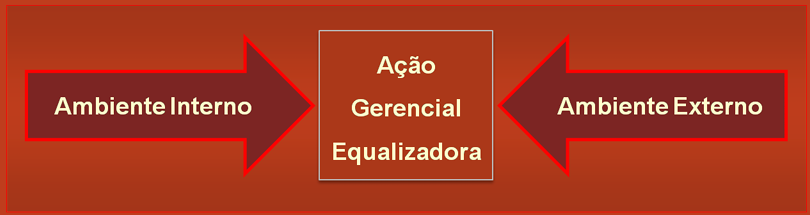
\includegraphics[width=0.5\textwidth]{img/imagem2.png}
    \label{fig:exemplo}
\end{figure}


A \textbf{cultura organizacional}, um componente crucial do ambiente interno, pode ser vista como a "personalidade" da organização. É definida como o sistema de valores e significados compartilhados pelos membros da organização, transmitidos por meio de histórias, rituais, lendas, símbolos, linguagem e cerimônias. A cultura diferencia uma organização de outra e se manifesta em aspectos como o estilo de liderança, a centralização ou descentralização da tomada de decisão e as práticas motivacionais.

A cultura organizacional desempenha um papel importante na adaptação da organização ao ambiente externo e na integração eficaz de seus processos internos. Ela reduz a ansiedade diante do desconhecido e da incerteza, impactando o desempenho da organização.

\begin{figure}[!h]
    \centering
    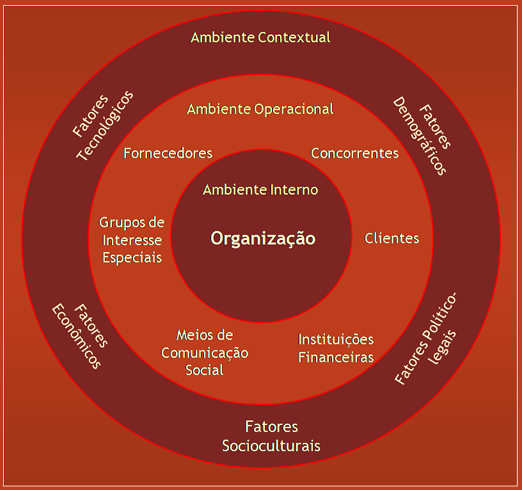
\includegraphics[width=0.5\textwidth]{img/imagem1.png}
    \label{fig:exemplo}
\end{figure}

\textbf{Culturas fortes}, onde os valores essenciais são amplamente compartilhados e seguidos, tendem a ter maior influência no comportamento dos membros da organização. Já em \textbf{culturas fracas}, os valores não são tão difundidos ou seguidos, resultando em menor impacto da cultura no comportamento.

É importante notar que a cultura organizacional também pode ser utilizada para ocultar e operacionalizar as relações de poder e dominação dentro da organização. Alguns autores defendem que a cultura deve ser analisada em conjunto com as manifestações de poder, considerando o papel da ideologia e do controle.

\section{O Ambiente Externo: Operacional e Contextual}
\begin{figure}[!h]
    \centering
    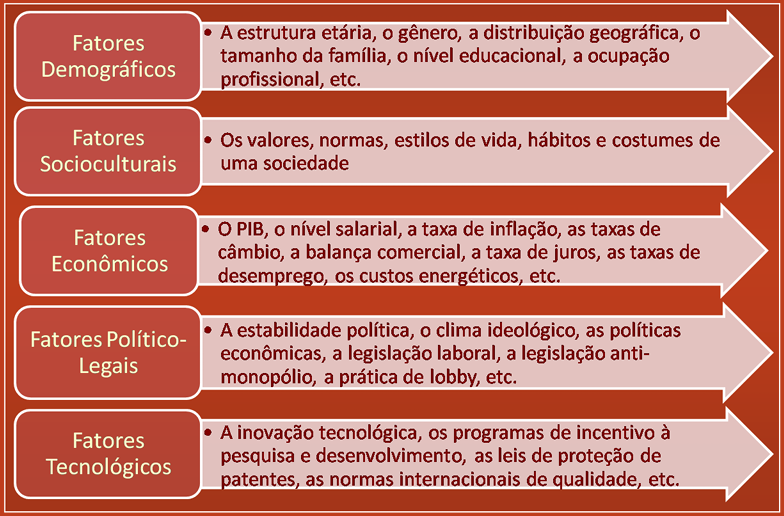
\includegraphics[width=0.5\textwidth]{img/imagem3.png}
    \label{fig:exemplo}
\end{figure}
O \textbf{ambiente externo} é o contexto no qual as organizações existem e operam, composto por elementos externos aos seus limites. Ele se divide em dois substratos: o ambiente contextual e o ambiente operacional.

\subsection{Ambiente Contextual}

O \textbf{ambiente contextual} inclui fatores externos que independem da ação da organização, como:

\begin{itemize}
    \item \textbf{Fatores econômicos:} Taxa de juros, inflação, PIB, etc.
    \item \textbf{Fatores político-legais:} Legislação, políticas governamentais, estabilidade política, etc.
    \item \textbf{Fatores socioculturais:} Valores, crenças, costumes da sociedade, etc.
    \item \textbf{Fatores demográficos:} Tamanho e composição da população, taxas de natalidade e mortalidade, etc.
    \item \textbf{Fatores tecnológicos:} Avanços tecnológicos, inovações, etc.
\end{itemize}

\begin{figure}[H]  % Use H para fixar a posição
    \centering
    \begin{minipage}{0.5\textwidth}
        \centering
        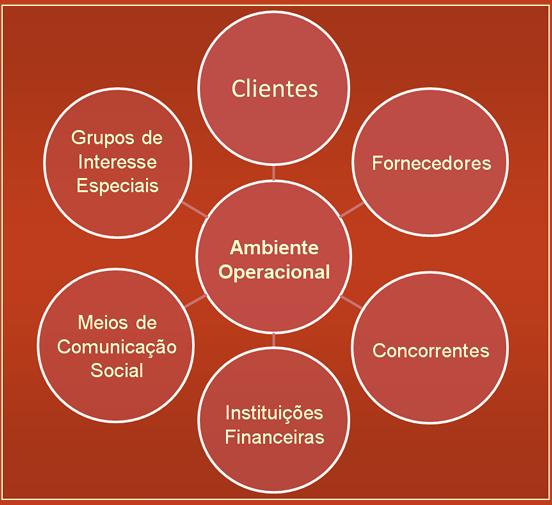
\includegraphics[width=\textwidth]{img/imagem4.png}
        \caption{Descrição da imagem}
        \label{fig:exemplo}
    \end{minipage}
\end{figure}


O ambiente contextual afeta as organizações indiretamente, influenciando o contexto geral em que operam.

\subsection{Ambiente Operacional}

O \textbf{ambiente operacional} é composto por elementos externos que interagem diretamente com a organização, influenciando seu desempenho de forma positiva ou negativa. Alguns exemplos são:

\begin{itemize}
    \item \textbf{Fornecedores:} Organizações que fornecem insumos e recursos para a empresa.
    \item \textbf{Clientes/Consumidores:} Aqueles que adquirem os produtos ou serviços da organização.
    \item \textbf{Concorrentes:} Organizações que competem pelos mesmos recursos e clientes.
    \item \textbf{Agências governamentais:} Órgãos reguladores e fiscalizadores.
    \item \textbf{Instituições financeiras:} Bancos, empresas de crédito, etc.
    \item \textbf{Meios de comunicação social:} Imprensa, redes sociais, etc.
    \item \textbf{Grupos de interesse especiais:} Sindicatos, ONGs, associações empresariais, etc.
\end{itemize}


A análise do ambiente operacional é crucial para que as organizações identifiquem oportunidades e ameaças e tomem decisões estratégicas para lidar com elas. Uma técnica comumente utilizada para essa análise é a \textbf{análise de stakeholders}, que consiste em identificar os grupos de interesse que afetam ou são afetados pelas ações da organização. Essa análise ajuda a entender os interesses e o poder de cada \textit{stakeholder}, permitindo que a organização desenvolva estratégias para gerenciar seus relacionamentos com eles.

É fundamental que as organizações compreendam a dinâmica entre o ambiente interno e o ambiente externo. A cultura organizacional e o ambiente externo se influenciam mutuamente, e a gestão eficaz dessa relação é essencial para o sucesso da organização.
